\subsection{Pequenas oscilações}\label{sec:3.5}
Agora já é possível analisar com detalhe as oscilações de energia de um elétron em um \textit{bunch}. Primeiramente, a análise será feita para o caso em que pequenas oscilações de energia causam também pequenas oscilações no deslocamento temporal $\tau$, as quais ocorrem desde que sejam limitadas por um pequeno intervalo correspondente a um segmento aproximadamente linear de $V(\tau)$. Na \autoref{sec:3.6} serão analisadas as oscilações não-lineares que ocorrem quando as variações de $\tau$ são grandes.

Para pequenos $\tau$ e $\epsilon$, pode-se substituir $v(\tau)$ e $U_{rad}(\epsilon)$ por suas aproximações lineares (séries de Taylor) contidas nas equações \eqref{eq:3.35} e \eqref{eq:3.23}, respectivamente. Assim, a equação \eqref{eq:3.34} fica
\begin{align}
	\frac{d\epsilon}{dt} = \frac{1}{T_0}(e\dot{V}_0 \tau - D\epsilon)\label{eq:3.40}
\end{align}
Esta equação pode ser combinada com a equação \eqref{eq:3.32}, resultando em uma equação diferencial para $\epsilon$ e $\tau$. Escolhendo $\tau$, pode-se tomar a derivada da equação \eqref{eq:3.32} com relação ao tempo e eliminar $\epsilon$, obtendo-se
\begin{align}
	\frac{d^2 \tau}{dt^2} + 2\alpha_\epsilon \frac{d\tau}{dt} + \Omega^2 \tau = 0\label{eq:3.41}
\end{align}
onde
\begin{align}
	\alpha_\epsilon &= \frac{D}{2 T_0}\label{eq:3.42}\\
	\Omega^2 &= \frac{\alpha\ e\ \dot{V}_0}{T_0\ E_0}
\end{align}

Note que a equação \eqref{eq:3.41} descreve uma oscilação harmônica amortecida com frequência angular de oscilação $\Omega$ e coeficiente de amortecimento $\alpha_\epsilon$. Como a taxa de amortecimento em um anel é sempre lenta ($\alpha_\epsilon<<\Omega$), a solução da equação \eqref{eq:3.41} pode ser escrita como
\begin{align}
	\tau(t) = A\ e^{-\alpha_\epsilon t}\ cos(\Omega t - \theta_0)
\end{align}
com $A$ e $\theta_0$ são constantes arbitrárias. Ou, usando a notação complexa usual,
\begin{align}
	\tau(t) = \tilde{\tau}\ e^{-(\alpha_\epsilon - i\Omega)t}
\end{align}
onde $\tilde{\tau}$ é uma constante complexa.

\begin{proof}
	Seja a variação de $\tau$ dada pela equação diferencial $\frac{d^2 \tau}{dt^2} + 2\alpha_\epsilon \frac{d\tau}{dt} + \Omega^2 \tau = 0$. Esta é uma EDO homogênea de segunda ordem, a qual pode ser resolvida através de sua equação característica:
	\begin{align*}
		r^2 + 2\alpha_\epsilon r + \Omega^2 = 0
	\end{align*}
	Resolvendo esta equação do segundo grau, tem-se que
	\begin{align*}
		r = \frac{-2\alpha_\epsilon \pm \sqrt{(2\alpha_\epsilon)^2 - 4\Omega^2}}{2}
	\end{align*}
	Considerando que $\alpha_\epsilon << \Omega$, pode-se simplificar a solução por
	\begin{align*}
		r = -\alpha_\epsilon \pm \Omega i
	\end{align*}
	Para uma equação característica com solução complexa, a solução da EDO é dada por
	\begin{align*}
		\tau = c_1\ e^{\alpha_\epsilon t}\ cos(\Omega t) + c_2\ e^{\alpha_\epsilon t}\ sen(\Omega t)
	\end{align*}
	Como um seno nada mais é que um cosseno defasado de $\pi/2$, esta solução pode ser reescrita como
	\begin{align*}
		\tau = A\ e^{\alpha_\epsilon t}\ cos(\Omega t - \theta_0)
	\end{align*}
\end{proof}

As equações \eqref{eq:3.40} e \eqref{eq:3.32} também podem ser resolvidas para $\epsilon$, obtendo-se a mesma equação diferencial \eqref{eq:3.41}. Assim, a variação de $\epsilon$ com o tempo é
\begin{align}
	\epsilon(t) = \tilde{\epsilon}\ e^{-(\alpha_\epsilon - i\Omega)t}
\end{align}
Pela equação \eqref{eq:3.32}, $\tilde{\epsilon}$ e $\tilde{\tau}$ são relacionados da seguinte maneira:
\begin{align}
	\tilde{\epsilon} = -i\frac{\Omega E_0}{\alpha}\tilde{\tau}\label{eq:3.47}
\end{align}
(considerando $\alpha_\epsilon << \Omega$) e, desta forma, as oscilações de $\epsilon$ e $\tau$ terão uma diferença de fase de $\pi/2$.

Note que a frequência de oscilação de pequenas oscilações de energia depende do sistema de Rf apenas pelo termo $\dot{V}_0$. A frequência é proporcional à raiz quadrada da derivada da RF na fase síncrona. Os outros parâmetros -- $\alpha$, $T_0$ $E_0$ -- são característicos do campo guia (incluindo a energia na qual ele é operado). A constante de amortecimento $\alpha_\epsilon$ das oscilações de energia -- a qual é o inverso da constante de amortecimento no tempo -- é proporcional a $D$, a qual é a taxa de variação da perda de energia por radiação. Como será mostrado posteriormente, esta taxa depende da energia do elétron e das propriedades do campo guia.

Para ajudar na análise dos resultados obtidos, é importante ter uma noção da ordem de magnitude das variáveis estudadas. Sendo assim, para um anel de armazenamento de 1 GeV:
\begin{align*}
	\omega_r = 2\pi /T_0 &\approx 10^7 s^{-1}\\
	\omega_\beta = \nu \omega_r &\approx 3\omega_r\\
	\Omega &\approx 10^4 s^{-1}\\
	\alpha_\epsilon &\approx 10 s^{-1}
\end{align*}
Analisando as relações $\omega_r/\Omega$ e $\Omega/\alpha_\epsilon$ pode-se justificar as aproximações feitas.

Na ausência de amortecimento, $\epsilon$ e $\tau$ são variáveis conjugadas. No diagrama de fase de $\epsilon$ versus $\tau$, as oscilações são descritas por um ponto que se move ciclicamente por uma elipse. Veja a \autoref{fig:fig35}(a). A relação entre os dois eixos principais da elipse é -- pela equação \eqref{eq:3.47}
\begin{align}
	\frac{\epsilon_{max}}{\tau_{max}} = \frac{|\tilde{\epsilon}|}{|\tilde{\tau}|} = \frac{\Omega E_0}{\alpha}
\end{align} 

\begin{figure}[!htb]
	\centering
	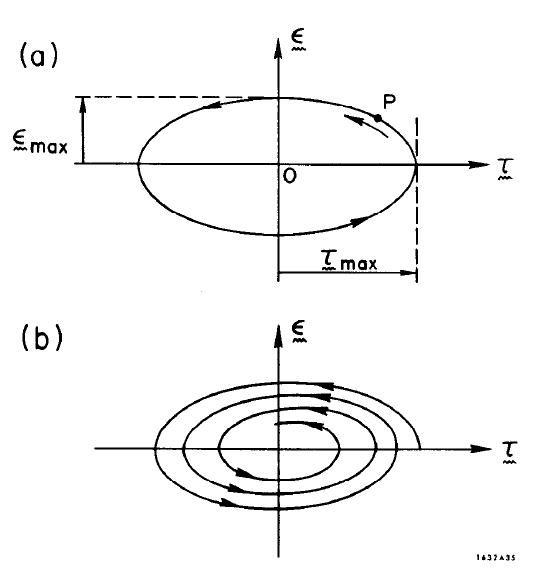
\includegraphics[width=0.6\linewidth]{./Figuras/fig35.jpeg}
	\caption{Diagrama de fase para as oscilações de energia. (a) Sem amortecimento. (b) Com amortecimento. (A taxa de amortecimento está bem exagerada). Retirado de \cite{sands1970physics}.}
	\label{fig:fig35}
\end{figure}

Se as escalas são escolhidas de forma que a elipse se torne um círculo, o ponto de referência rotaciona a uma frequência angular $\Omega$ constante. Com amortecimento, o tamanho da elipse decresce lentamente e a fase da trajetória é uma lenta espiral convergindo para o centro, como pode-se ver na \autoref{fig:fig35}(b). O diagrama de fase também mostra porque o amortecimento depende de $dU_{rad}/dE$. Se sua derivada é positiva, o elétron está perdendo uma quantidade extra de energia na metade superior da elipse, e ganhando uma quantidade extra de energia na metade inferior. Desta forma, o ponto de referência está sempre se dirigindo para o eixo $\tau$ e a amplitude de oscilação está diminuindo -- proporcionalmente a $dU_{rad}/dE$.

De acordo com a solução aqui proposta, as oscilações de energia de todos os elétrons deveriam ser completamente amortecidas em algum momento, fazendo com que todos os elétrons fiquem sobre o elétron síncrono. Mas ainda não foi considerada a excitação das oscilações causada por efeitos quânticos os quais "balançam" as oscilações e previnem que estas sejam completamente anuladas (estes efeitos serão considerados na \autoref{part4}). Em condições estacionárias, qualquer elétron armazenado será tipicamente encontrado com uma amplitude de oscilação residual na qual há um balanço entre a excitação e o amortecimento. Como ambos os processos são lentos, pode-se pensar que a oscilação de energia em qualquer curto período de tempo pode ser descrita por uma elipse fixa, como a representada na \autoref{fig:fig34}(a).

É importante ter em mente que as oscilações de energia estão relacionadas não só com as oscilações longitudinais (em $y$ ou $\tau$) dos elétrons em um \textit{bunch}, mas elas também possuem uma componente lateral. De acordo com a equação \eqref{eq:3.3}, o desvio de energia $\epsilon$ resulta em um deslocamento radial $x_\epsilon$ proporcional a $\epsilon$ -- e em fase com o mesmo. Então a componente $x_\epsilon$ do deslocamento horizontal total oscila em sincronia com as oscilações de energia. Em geral, esta manifestação transversal das oscilações de energia possui (em condições estacionárias) uma amplitude muito próxima das oscilações betatron.